\section {数式処理を用いたコードとドキュメントの自動生成}
\label {sec: solution}

本節は数学的知識を背景にした領域の記述について,数式処理システムを利用することが有効であること,特に,前節において挙げた平方根の問題がエレガントに記述できることを示す.

\subsection {Jupyter/Pythonプログラマのための数式処理システムSymPy}

SymPyは数式処理を実施するためのPythonライブラリである.数式処理システムとしては,既存のReduce, Maple, Mathematicaに比べると不十分な点は多いが,Pythonを用いたソフトウェア開発の面からは面白い興味深い点がある.

既存の数式処理システムとは異なりSymPyはライブラリであり,プログラミング言語ではない.すなわち,SymPyを利用することによって,数式を表現するためのデータ構造と数式上の演算を表現する各種関数や演算子が利用できるようになる.SymPyを用いることで数学記号と重要な定数,関数,等式や不等式,行列やテンソル,方程式系などが表現できる.これらはPythonのデータ構造として提供されるため,標準的なPythonのデータ構造と同様にPythonの変数に束縛したり,Pythonの関数に実引数として渡すことができる.

数式に対しては一般的な代数演算や微積分を施すことができる.また,方程式系のソルバーは与えられた方程式系の解析的な解を与える.たとえば,以下の例では二つの数学の変数$a$と$x$を用意し,それぞれPythonの変数\verb|a|と\verb|x|に束縛した上で,簡単な数式$(x^2 - a)$を作成したものを(数式)微分した結果として$2x$を得ている.

\bgroup \color {darkred}
\begin{verbatim}
$ python -q
>>> import sympy
>>> a, x = sympy.var('a x')
>>> e = x**2 - a
>>> e.diff(x)
2*x
>>> f = sympy.lambdify([x], e.diff(x))
>>> f(5)
10
\end{verbatim}
\egroup

%$

Pythonプログラマにとって有り難い存在として,SymPyで表現した数式に相当するPythonのラムダ式を生成する機能(\verb|lambdify|)がある.このように生成されたラムダ式を用いれば,SymPyの数式に該当する数値計算ができる.上の例では\verb|lambdify|を用いて\verb|e.diff(x)|を変換してPythonの関数\verb|f|を得,\verb|f(x)|が確かに10を返すことを確認している.

\begin {figure}[tb]
  \rule {\linewidth} {1pt}
  \bgroup \small \color {darkred}
  \verbatiminput {code/md.py} \egroup

  \caption {SymPy形式の数式が混ざったテキスト列からMarkdown文書を生成するユーティリティの定義}
  \label {fig: md function}
  \rule {\linewidth} {1pt}
\end {figure}

さらにドキュメントを書くときに有用なのはSymPyで表現した数式を\LaTeX{}形式の文字列に変換する機能である.

\bgroup \color {darkred}
\begin{verbatim}
>>> sympy.latex(e)
'- a + x^{2}'
\end{verbatim}
\egroup

この機能を利用することで,ドキュメント記述の文字列とSymPy形式の数式が混在するデータ列から,MathJax拡張を施したMarkdown書式のドキュメントを生成するためのユーティリティ関数\verb|md|を定義した.(図\ref {fig: md function})

\begin {figure}[tb]
  \rule {\linewidth} {1pt}
  \bgroup \small \color {darkred}
  \verbatiminput {code/sqrt1.py} \egroup

  \caption {Newton-Raphson法の一般的な記述}
  \label {fig: newton raphson implementation}
  \rule {\linewidth} {1pt}
\end {figure}

\begin {figure}[tb]
  \rule {\linewidth} {1pt}
  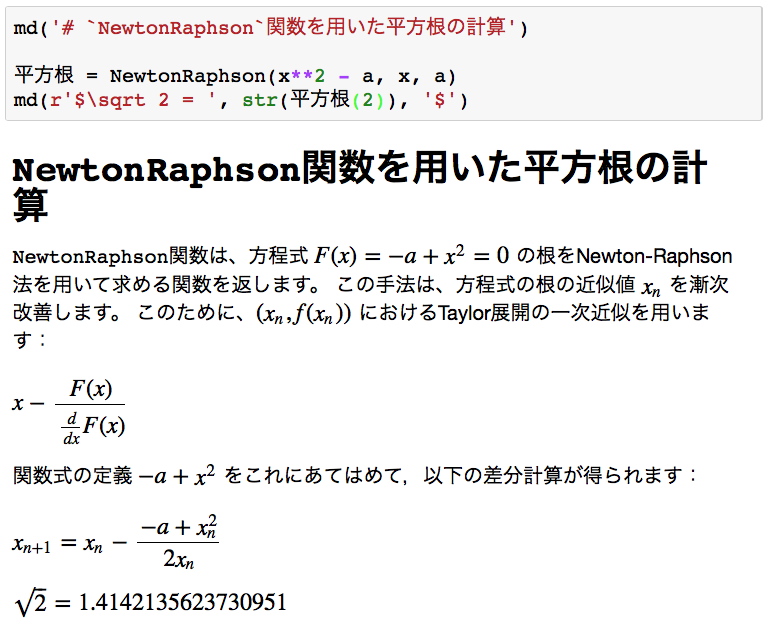
\includegraphics [width=\linewidth] {newton-raphson.png}

  \caption {図\ref {fig: newton raphson implementation}を用いて,平方根を計算する関数を生成し,$\sqrt 2$を計算させた様子.平方根が正しく計算されているだけでなく,平方根を計算する内部ドキュメントは\ref {fig: newton raphson documentation}の記述を平方根の計算に特殊化させたものが生成されている.}
  \label {fig: square root generated}
  \rule {\linewidth} {1pt}
\end {figure}

前節においてはNewton-Raphson法を用いて平方根を計算するプログラムを紹介した.これに対して図\ref {fig: newton raphson implementation}は,平方根に限定せずNewton-Raphson法を一般的に記述したプログラムである.この関数は,引数として根を求めたい方程式(関数式)とその方程式における変数(\verb|x|)を受け取り,与えられた方程式を\verb|x|で受け取った(数学の)変数について求解する関数を返す.

\begin {figure}[tb]
  \rule {\linewidth} {1pt}
  {\color {darkblue} \small \verbatiminput{code/sqrt1.md}}
  \caption {図\ref {fig: newton raphson implementation}の内部ドキュメント記述}
  \label {fig: newton raphson documentation}
  \rule {\linewidth} {1pt}
\end {figure}

たとえば,関数式として\verb|x**2 - a|を与えると,方程式$x^2 - a = 0$を数値的に求解するPython関数,すなわち平方根を計算する関数を返す.図\ref {fig: square root generated}では,こうして得られたPython関数を「平方根」という名前のPython変数に束縛した上で,引数に2を渡すことで,$\sqrt {2}$の近似解として$1.41421356\ldots$を得ている.

では,図\ref {fig: newton raphson implementation}の記述を見ていこう.引数に与えられた関数式と変数\verb|x|はそれぞれSymPy表現の数式と数学記号である.3行目で定義されたPython変数には,Newton-Raphson法の差分式($x - F(x) / F'(x)$)がSymPyの数式として与えられ,Python変数の\verb|NR|\footnote {NRはNewton-Raphsonを短縮した名前.}で束縛している.ここまでは関数の形を特定せずに表現してきたが,実際には\verb|NewtonRaphson|関数の引数「関数式」として,たとえば$x^2 - a$のような数式が与えられる.そのことを反映するために,一般的な差分式の$F(x)$を具体的な関数式の内容で置き換えている操作を経て,\textbf {差分計算式}を定義している.差分計算式を方程式の変数$x$によって抽象化したものが差分を数値計算する\textbf {差分計算}関数である.

\verb|newton_raphson|関数のなかでは,このように得た\textbf {差分計算}関数を繰り返し呼び出すことでNewton-Raphson法の計算を実施している.最終的に\verb|NewtonRaphson|関数は\verb|newton_raphson|関数を返り値として与える.ここで返される\verb|newton_raphson|関数は,一般的なNewtonRaphson法の計算を引数に与えた関数式に関して特殊化したものと見做すことができる.

ここでの実装は,Newton-Raphson法の(特定の数式の例の依らない)一般的な記述(図\ref {fig: newton raphson implementation})と平方根を求めるためにNewton-Raphson法を方程式$x^2 -a = 0$適用する記述(図\ref {fig: square root generated})にきれいに分離されている.前者は,Newton-Raphson法の方式を素直な数式処理として記述したものである.後者は\verb|NewtonRaphson|関数に\verb|x**2 - a|というまさに平方根を定義する式を受け渡すのみである.以上より\ref {ssec: definition}節で指摘した平方根の定義式が消え失せる問題が解消されるだけでなく,元々の記述のなかでNewton-Raphson法の一般的な性質と平方根という特定の応用問題の記述が混在していた問題も解消できた.

さて,図\ref {fig: newton raphson documentation}は,図\ref {fig: newton raphson implementation}に対応したドキュメントを生成するコードである.このコードを図\ref {fig: newton raphson implementation}の\textbf {return}文の直前に挿入することによって,\verb|NewtonRaphson|を\textbf {関数式}の内容に特化したドキュメントを生成できる.

この記述において,注目すべき点は図\ref {fig: square root document description}と比較して数式の記述量が大幅に少ない点である.これは,\verb|NewtonRaphson|関数の定義に出現するSymPy表現の4つの数式(\verb|F(x)|,関数式,\verb|NEWTON_RAPHSON|,\verb|差分計算式|)を埋め込むことによって,それらを具体的に記述する手間が除去されているからである.この結果,\ref {ssec: complexity}で指摘されたドキュメント記述の複雑性の問題を避けることができた.

このことは単なる記述の簡素化と理解してはいけない.もうひとつの重要な点は,プログラム記述とドキュメント記述の間の冗長性が除去されていることである.以前のドキュメント記述(図\ref {fig: square root document description})にはさまざまな数式が具体的な形で出現していた.一方,今度のドキュメント記述では,具体的な数式の構成はSymPy数式を扱う\verb|NewtonRaphshon|関数の記述や,図\ref {fig: square root generated}に現れるSymPy表現の数式を活用している.

このことはプログラムコード記述に出現する数式を表現したデータ構造を活用し,ドキュメントに出現する数式の生成に用いることによって,データ構造として表現された数式の再利用性を高めて,プログラムコード記述とドキュメント記述の双方で利用したと見做せる.この結果\ref {ssec: redundancy}節で指摘した数式記述の冗長性の問題を解決できた.
